\documentclass[pdf]{beamer}
\usepackage[utf8]{inputenc}
\usepackage{graphicx}
\usepackage[export]{adjustbox}

\mode<presentation>{\usetheme{Warsaw}}
\setbeamertemplate{footline}[frame number]
\setbeamertemplate{caption}[numbered]
\usefonttheme[onlymath]{serif}
\AtBeginSection[]
{
\begin{frame}{Table of Contents}
\tableofcontents[currentsection]
\end{frame}
}

\title{\textbf{A Practical Analysis of the Convergence of Back Propagation}}
\author{
  Andrei~Purcarus \and Sean~Stappas
}
\institute{
  ECSE 526 \\
  McGill University
}
\date{November 30, 2017}

\begin{document}

\maketitle

\begin{frame}
\frametitle{Table of Contents}
\tableofcontents
\end{frame}


\section{Objectives}

\begin{frame}
\frametitle{Objectives}
\begin{itemize}
  \item Implement a fully connected neural network.
  \item Analyze the effects on performance and convergence of several improvements to back propagation, including those proposed by LeCun's 1998 paper \textit{Efficient BackProp} \cite{lecun_efficient_1998}.
  \item Perform practical tests on the MNIST data set.
\end{itemize}
\end{frame}
\begin{frame}

\frametitle{MNIST}
\begin{figure}[!htb]
  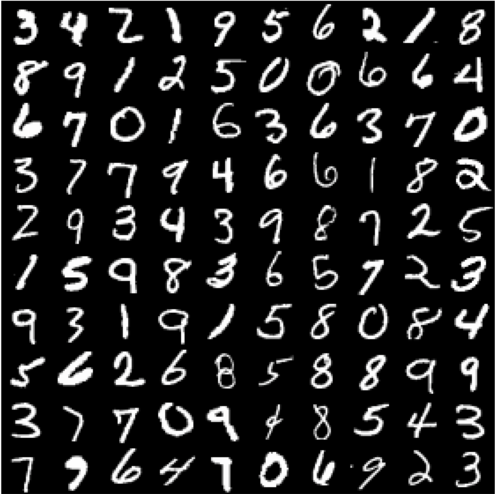
\includegraphics[height=0.7\textheight]{figures/mnist.png}
  \caption{Sample digits from the MNIST dataset \cite{steeves_2015}.}
\end{figure}
\end{frame}

\section{Design Methodology and Results}

\begin{frame}
\frametitle{Input Normalization}

Average of the input training data should be close to 0.

\begin{equation}
x \leftarrow x - \bar{x}
\end{equation}

Variance of the input training data should be the same for each feature ($\approx 1$).

\begin{equation}
x_i \leftarrow \frac{x_i}{\sigma_{x_i}}
\end{equation}

\end{frame}

\begin{frame}
\frametitle{Sigmoid}
Logistic sigmoid:
\begin{equation}
  f_{logistic}(x) = \frac{1}{1 + e^{-x}}
\end{equation}
Tanh sigmoid:
\begin{equation}
  f_{tanh}(x) = 1.7159 \tanh \left( \frac{2}{3} x \right)
\end{equation}
\begin{itemize}
  \item Symmetric about the origin.
  \item $f(\pm1) = \pm1$.
  \item Second derivative maximum at $x=1$.
  \item Output variance close to 1 if input is normalized.
\end{itemize}
\end{frame}

\begin{frame}
\frametitle{Sigmoid}
\begin{figure}[!htb]
  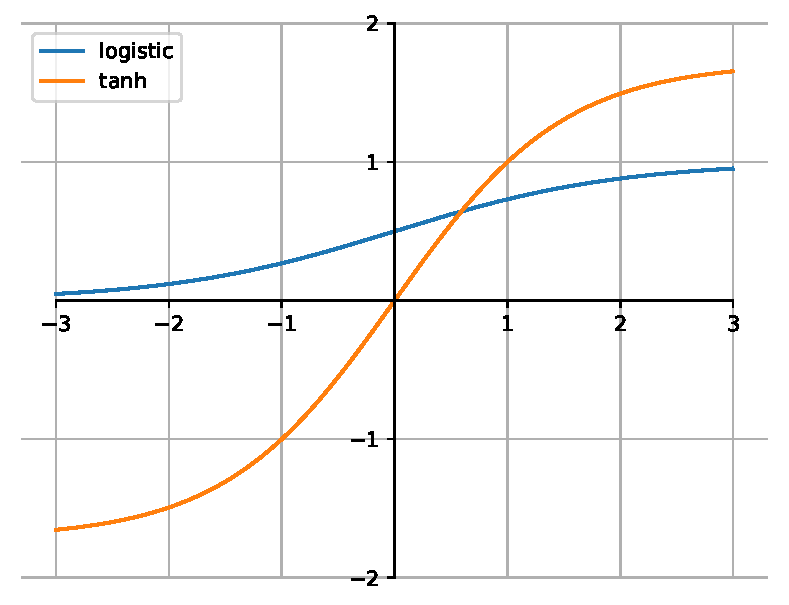
\includegraphics[height=0.8\textheight]{plots/logistic_vs_tanh_function.pdf}
\end{figure}
\end{frame}

\begin{frame}
\frametitle{Sigmoid}
\begin{figure}[!htb]
  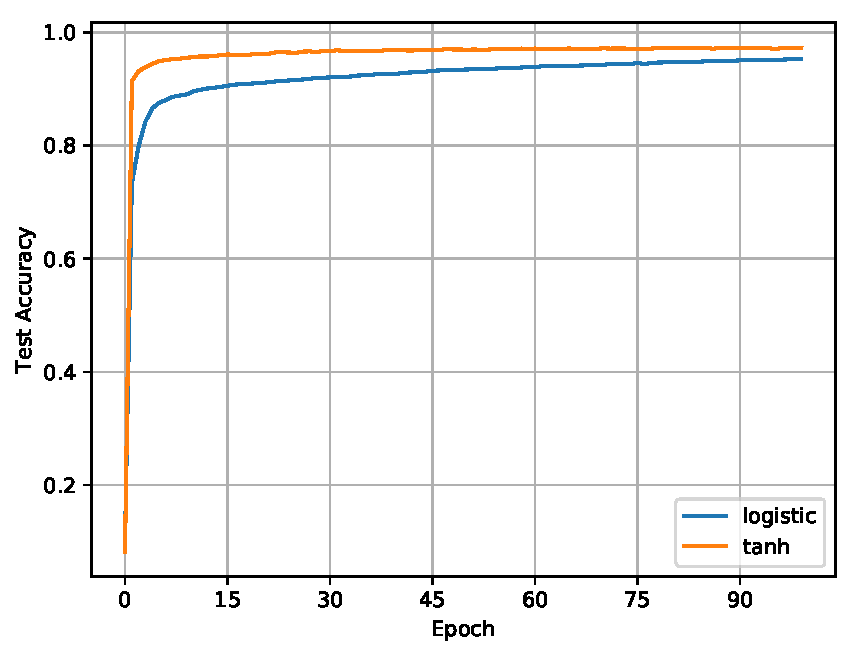
\includegraphics[height=0.8\textheight]{plots/logistic_vs_tanh.pdf}
\end{figure}
\end{frame}

\begin{frame}
\frametitle{Weight Initialization}

Initial weights should be randomly drawn from a distribution with zero mean and standard deviation $\sigma_w$ ($m$: fan-in).

\begin{equation}
  \sigma_w = m^{-1/2}
\end{equation}

This ensures that the initial weights range over the sigmoid's linear region (assuming input normalization and tanh sigmoid).

\begin{itemize}
\item Gradients large enough for learning to proceed.
\item Linear learning occurs before more difficult nonlinear learning.
\item Distribution of outputs of each node has $\sigma \approx 1$.
\end{itemize}
\end{frame}

\begin{frame}
\frametitle{Learning Rate}
\begin{equation}
  w_i \leftarrow w_i - \eta_i \frac{\partial E}{\partial w_i}
\end{equation}
\begin{itemize}
\item $\eta_i$: learning rate for weight $w_i$.
\item Large learning rate: oscillations.
\item Small learning rate: slow learning.
\end{itemize}
\end{frame}

\begin{frame}
\frametitle{Learning Rate}
\begin{figure}[!htb]
  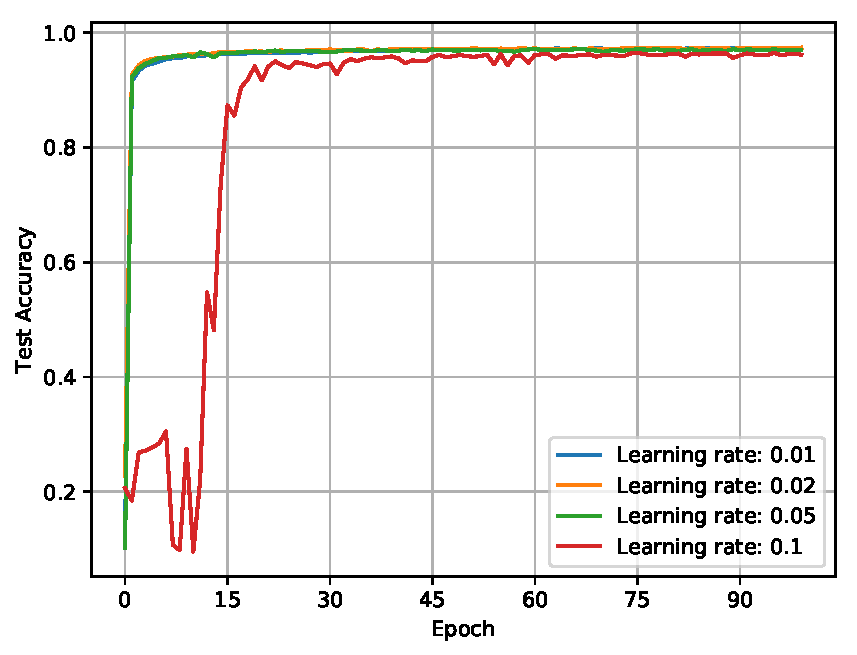
\includegraphics[height=0.8\textheight]{plots/learning_rate.pdf}
\end{figure}
\end{frame}

\begin{frame}
\frametitle{Learning Rate}
\begin{figure}[!htb]
  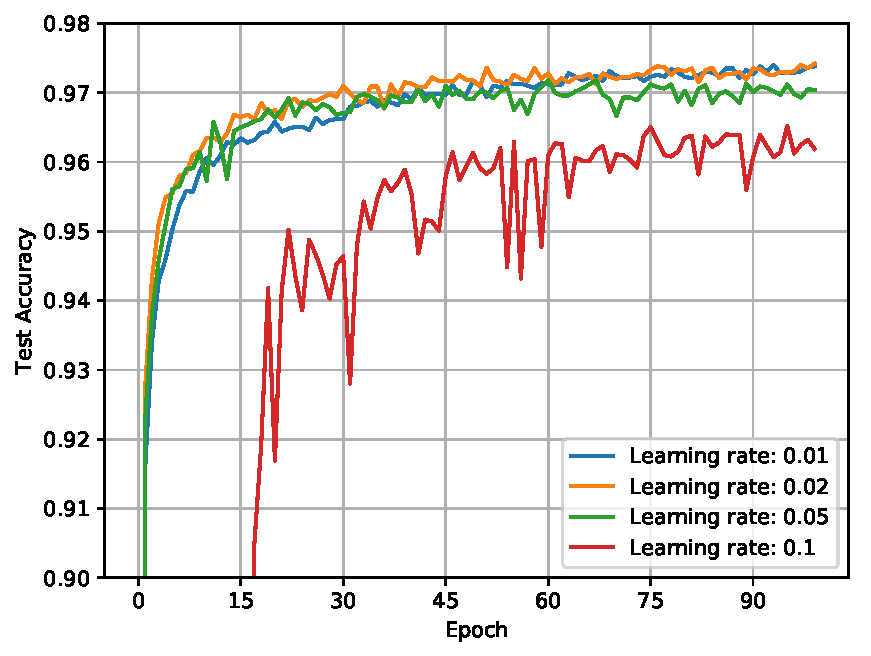
\includegraphics[height=0.8\textheight]{plots/learning_rate_zoom_2.pdf}
\end{figure}
\end{frame}

\begin{frame}
\frametitle{Layer Decay}

Learning rate for weights in lower layers should be larger than for those in higher layers.

\begin{equation}
  \eta_i = \delta \eta_{i-1}
\end{equation}

\begin{itemize}
\item $\eta_i$: learning rate in layer $i$ (layer $i$ is higher than layer $i-1$).
\item $\delta$: layer decay ($0 < \delta \leq 1$).
\end{itemize}

\end{frame}

\begin{frame}
\frametitle{Layer Decay}
\begin{figure}[!htb]
  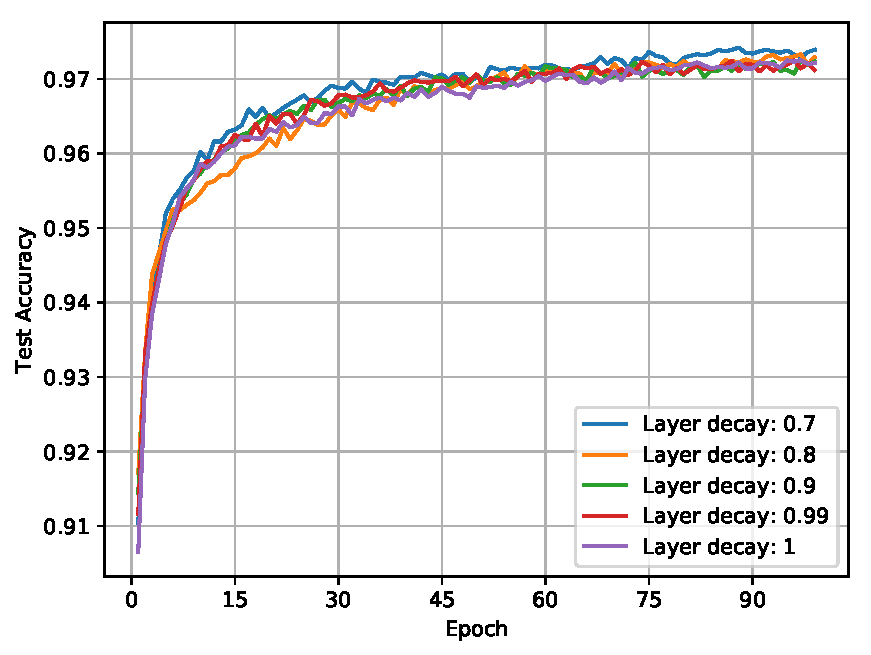
\includegraphics[height=0.8\textheight]{plots/layer_decay_zoom.pdf}
\end{figure}
\end{frame}

\begin{frame}
\frametitle{Momentum}
\begin{equation}
  \Delta w(t + 1) \leftarrow - \eta \nabla E + \mu \Delta w(t)
\end{equation}
\begin{itemize}
  \item $\mu$: momentum.
  \item Avoids getting stuck in local minima.
  \item Large momentum: overshoot the minimum.
  \item Small momentum: slow learning.
\end{itemize}
\end{frame}

\begin{frame}
\frametitle{Momentum}
\begin{figure}[!htb]
  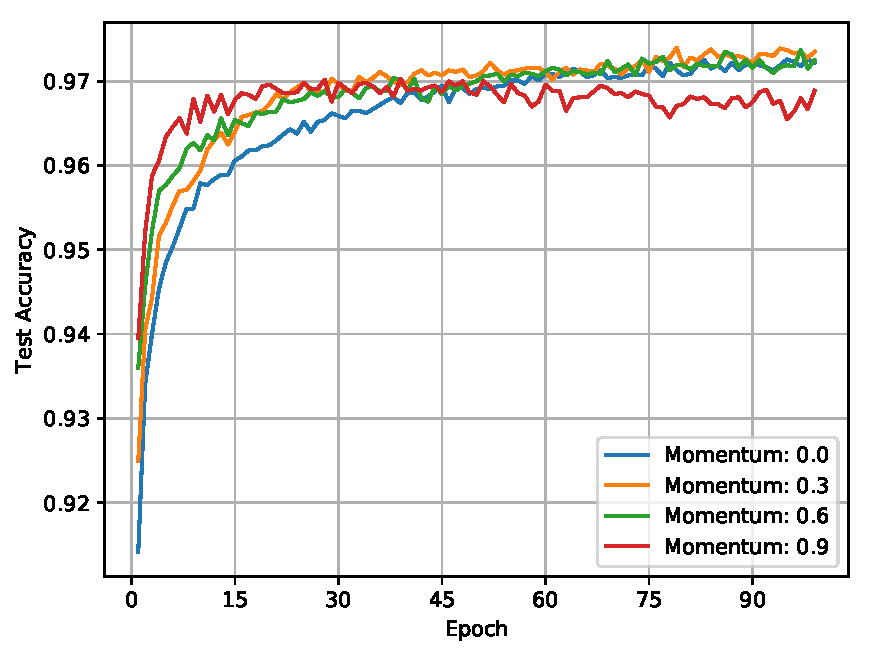
\includegraphics[height=0.8\textheight]{plots/momentum_zoom.pdf}
\end{figure}
\end{frame}

\begin{frame}
\frametitle{Batch Size}
\begin{figure}[!htb]
  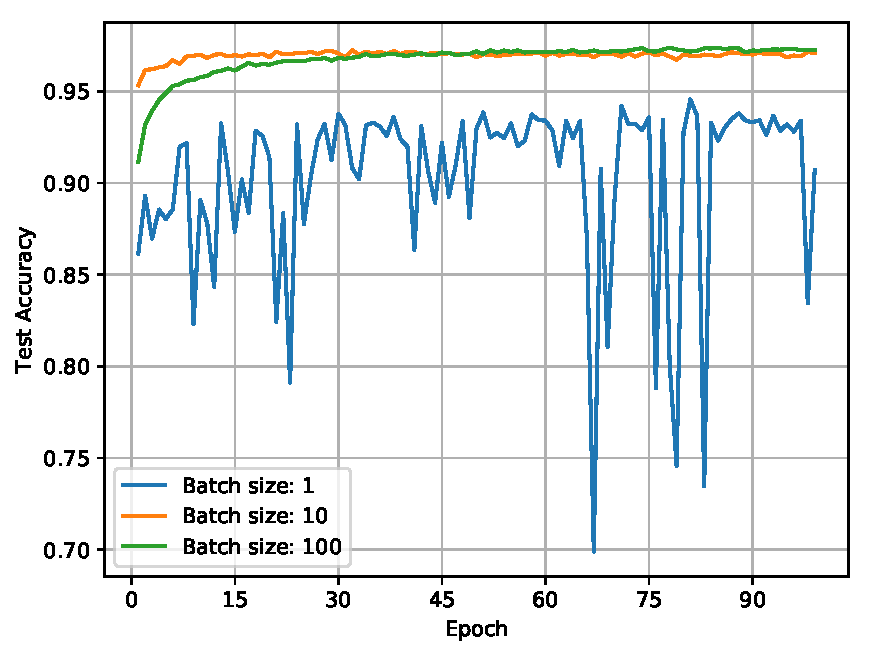
\includegraphics[height=0.8\textheight]{plots/batch_size_zoom.pdf}
\end{figure}
\end{frame}

\begin{frame}
\frametitle{Layer Sizes}
\begin{figure}[!htb]
  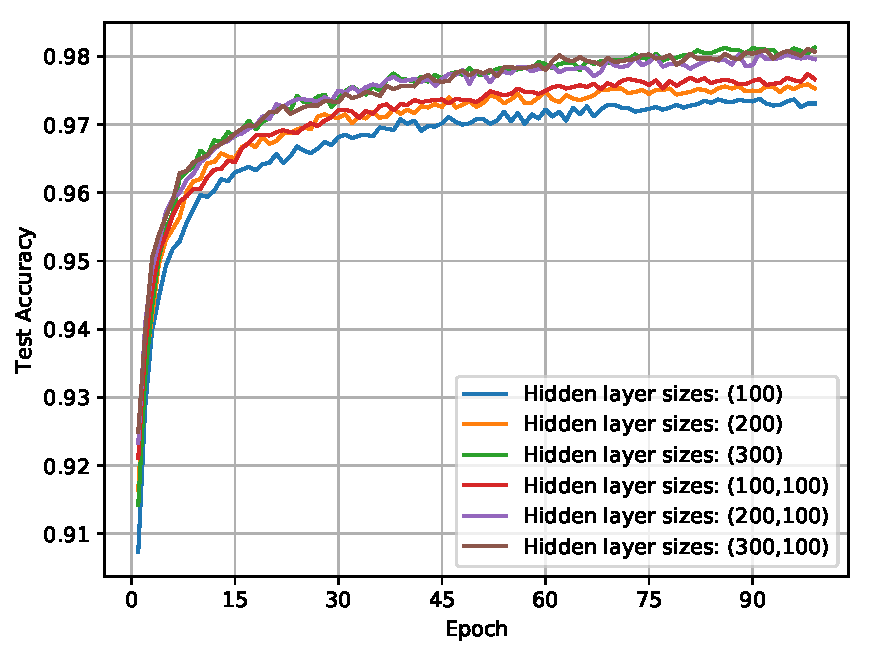
\includegraphics[height=0.8\textheight]{plots/network_size_zoom.pdf}
\end{figure}
\end{frame}

\begin{frame}
\frametitle{Comparison to Other Approaches}
\begin{itemize}
  \item Deep convolutional network using TensorFlow \cite{tensorflow}.
  \item Learns localized features of the input.
  \item Learned features are translation invariant.
  \item Better for image recognition problems (like MNIST).
\end{itemize}
\end{frame}

\begin{frame}
\frametitle{Comparison to Other Approaches}
\begin{figure}[!htb]
  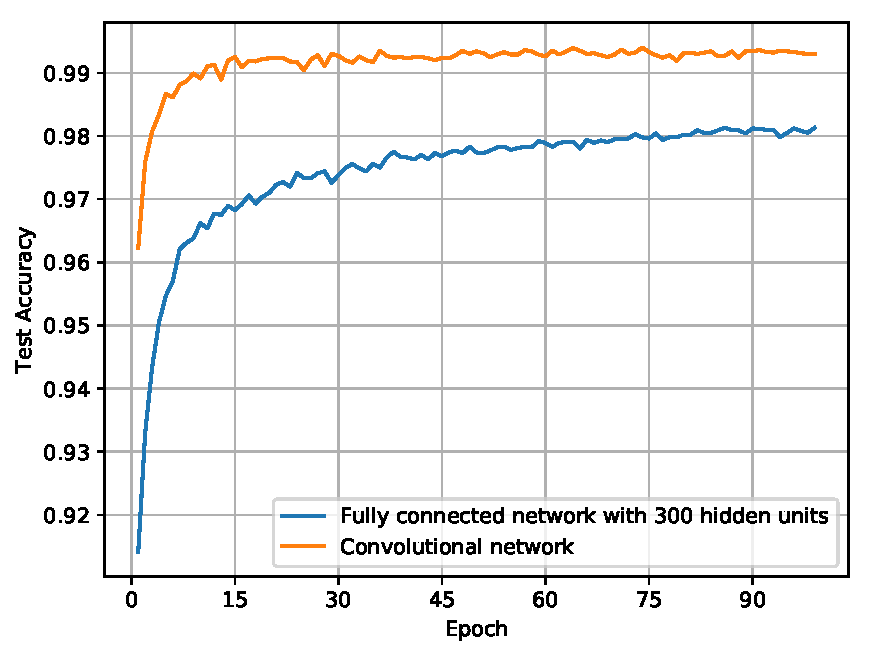
\includegraphics[height=0.8\textheight]{plots/network_comparison.pdf}
\end{figure}
\end{frame}

\section{Demo}

\begin{frame}
\frametitle{Demo}
\begin{itemize}
  \item Inspired by the OCHRE applet \cite{ochre}.
\end{itemize}
\begin{figure}[!htb]
  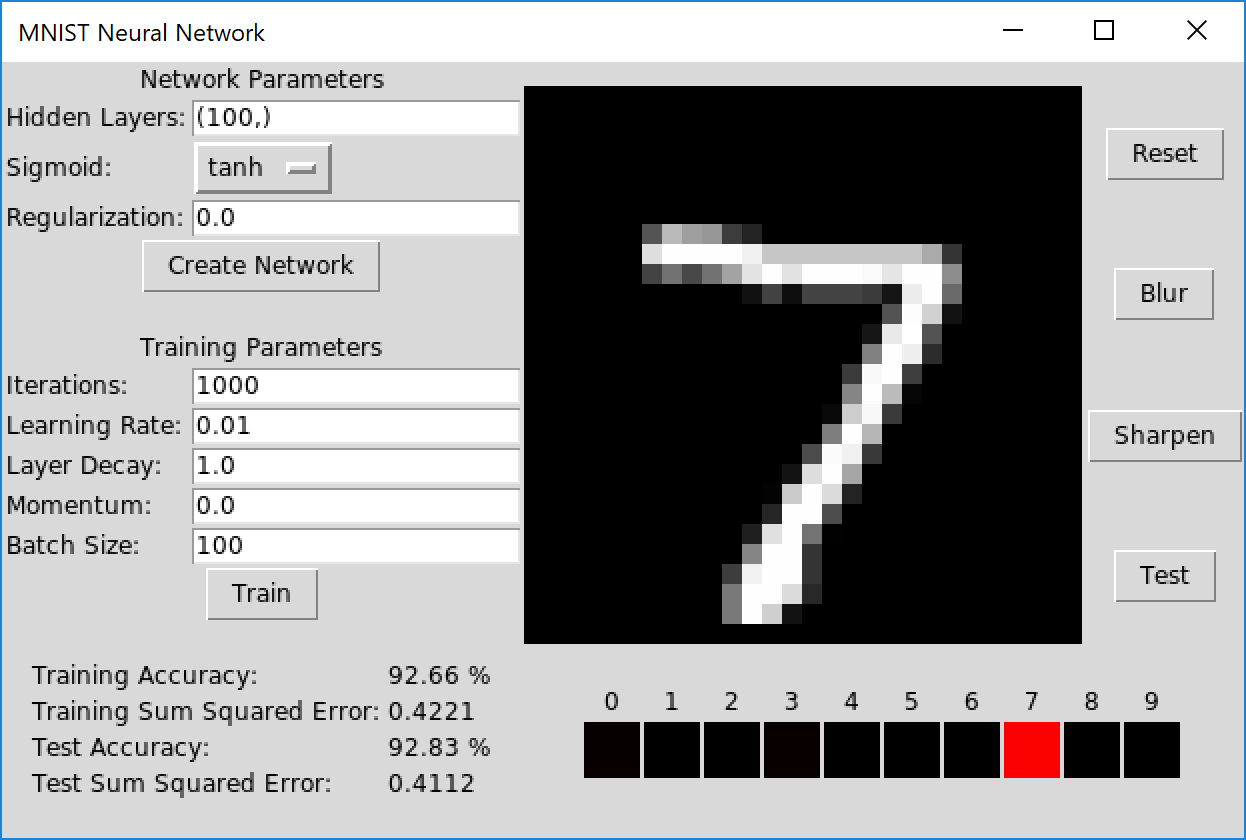
\includegraphics[height=0.6\textheight]{figures/gui.png}
\end{figure}
\end{frame}

\section{References}

\begin{frame}
\bibliographystyle{IEEEtran}
\bibliography{IEEEabrv,references}
\end{frame}

\end{document}
